\section{Procedure and Analysis}

\subsection{Initiation and characteristics of the laser diode}

After switching on the laser diode and the thermoelectric cooler, we controlled the progression and the coherence of the laser beam and verified the correct position of the lenses, so that the beam focused on the detector of the photodiode. We did this by using an infrared display unit and a white piece of paper in order to be able to see the actual progression of the beam.\\

We then turned on the photodiode and the preamplifier, which we set to DC and the gain to 40 dB. We installed the etalon into the optical path and set it perpendicular to the beam. The laser was modulated by a sawtooth voltage in order to be able to see a few wavelength-peaks of the etalon.\\

In the first part of this measurement, the current of the diode was held at a constant value of $I = (35.1\pm 0.3)\ mA$ while the temperature was varied from $34.0^\circ C$ to $36.5^\circ C$. We measured the scrolling of the peaks in dependence of the temperature.
In the second part of the measurement, we held the temperature constant at a value of $T=(34.7 \pm 0.2)\ ^\circ C$ and changed the current from 20.4 to 36.7 mA.
Our measurements were okay, but left room for improvement, which we did in the second week, with the following adjustments:\\

\begin{center}
\begin{tabular}[H]{l l c}
Constant Temperature & \\
Temperature & $T=34.7 ^\circ C$\\
Current & $I = 54.0 \dots 69.0\ mA$\\
 & \\
Constant Current & \\
Laser Current & $I = 64.4 mA$\\
Temperature & $T=32.3 \dots 33.65\ ^\circ C$\\
\end{tabular}
\end{center}

For both measurements, we followed one peak and measured its position in dependence of the current or the temperature of the laser diode. We used the distance of the different peaks to calculate the calibration factor $f$ between the relative position $\Delta t$ and the relative frequency $\nu$ of the peak. It is given by

$$ f = \frac{FSR}{\Delta t} \ \ \ \ \ \text{with the error}\ \ \ \ \ \frac{s_f}{f} \approx \frac{s_{FSR}}{FSR} = 3.00 \cdot 10^{-3} $$

where FSR is the free spectral range of the etalon, whose numerical value is $FSR = (9924 \pm 30)\ MHz$. The error $s_t$ is negligible. The frequency is the given by:

$$\nu = f\cdot t \ \ \ \ \ \text{with the error}\ \ \ \ \ \frac{s_\nu}{\nu} \approx \frac{s_f}{f} = 3.00 \cdot 10^{-3} $$

\subsubsection{Constant Temperature}

By measuring the distance between two peaks we were able to calculate the calibration factor between time and frequency.

$$f = (70.886 \pm  0.214) \frac{MHz}{\mu s} $$

We then were able to plot the relative frequency in dependence of the variation of the laser current and by linear regression find out their relation.

\begin{figure}[H]
\centering 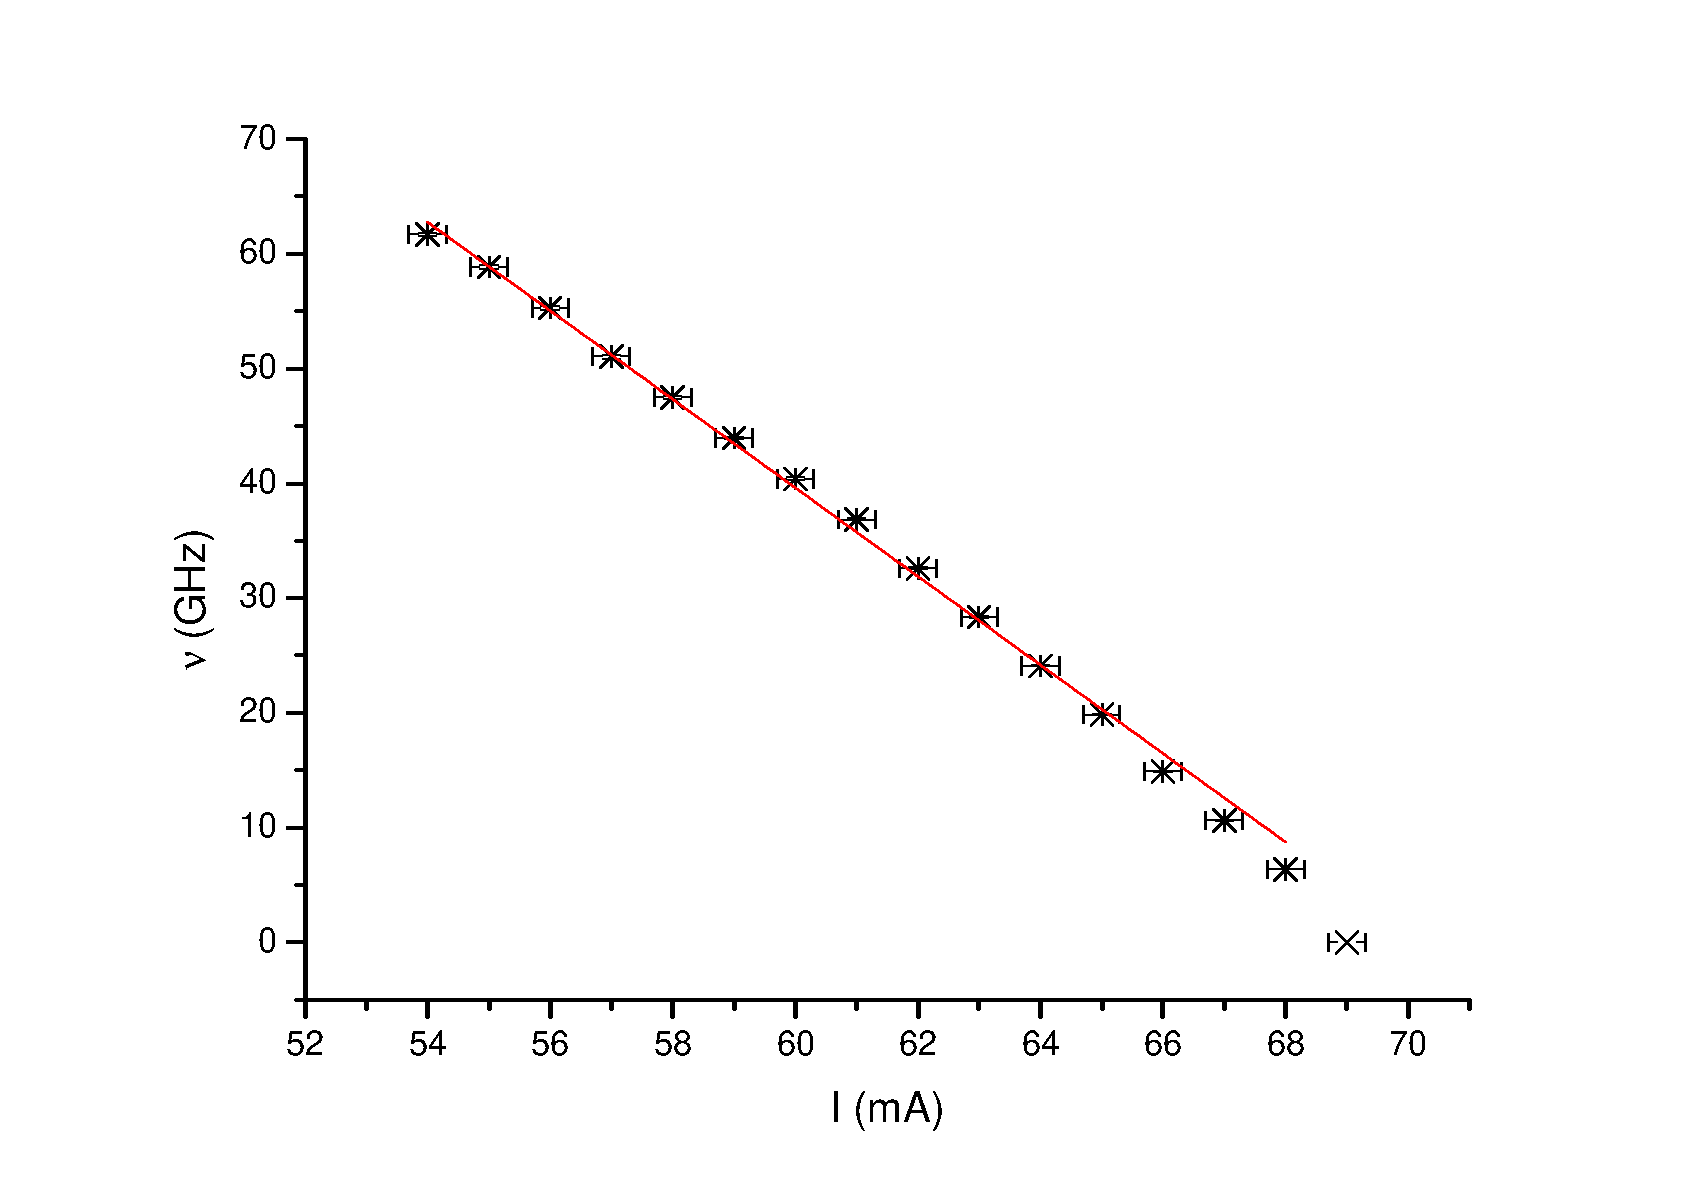
\includegraphics[width=0.9\textwidth]{BilderAusw/T_fest.pdf}
\caption{Variation of the laser current with constant temperature}
\end{figure}

As one can see, the slope is negative, which means that by increasing the current, the light emitted by the laser has a lower frequency. We find that the slope is

$$ a = (-3.858 \pm 0.056)\ \frac{GHz}{mA}$$

which is the conversion factor between the frequency $\nu$ of the laser light and the current $I$ of the diode.

\subsubsection{Constant Current}

The calibration gave us the same conversion factor as before, i.e.

$$f = (70.886 \pm  0.214) \frac{MHz}{\mu s} $$

and we plotted the relative frequency in dependence of the temperature of the laser.

\begin{figure}[H]
\centering 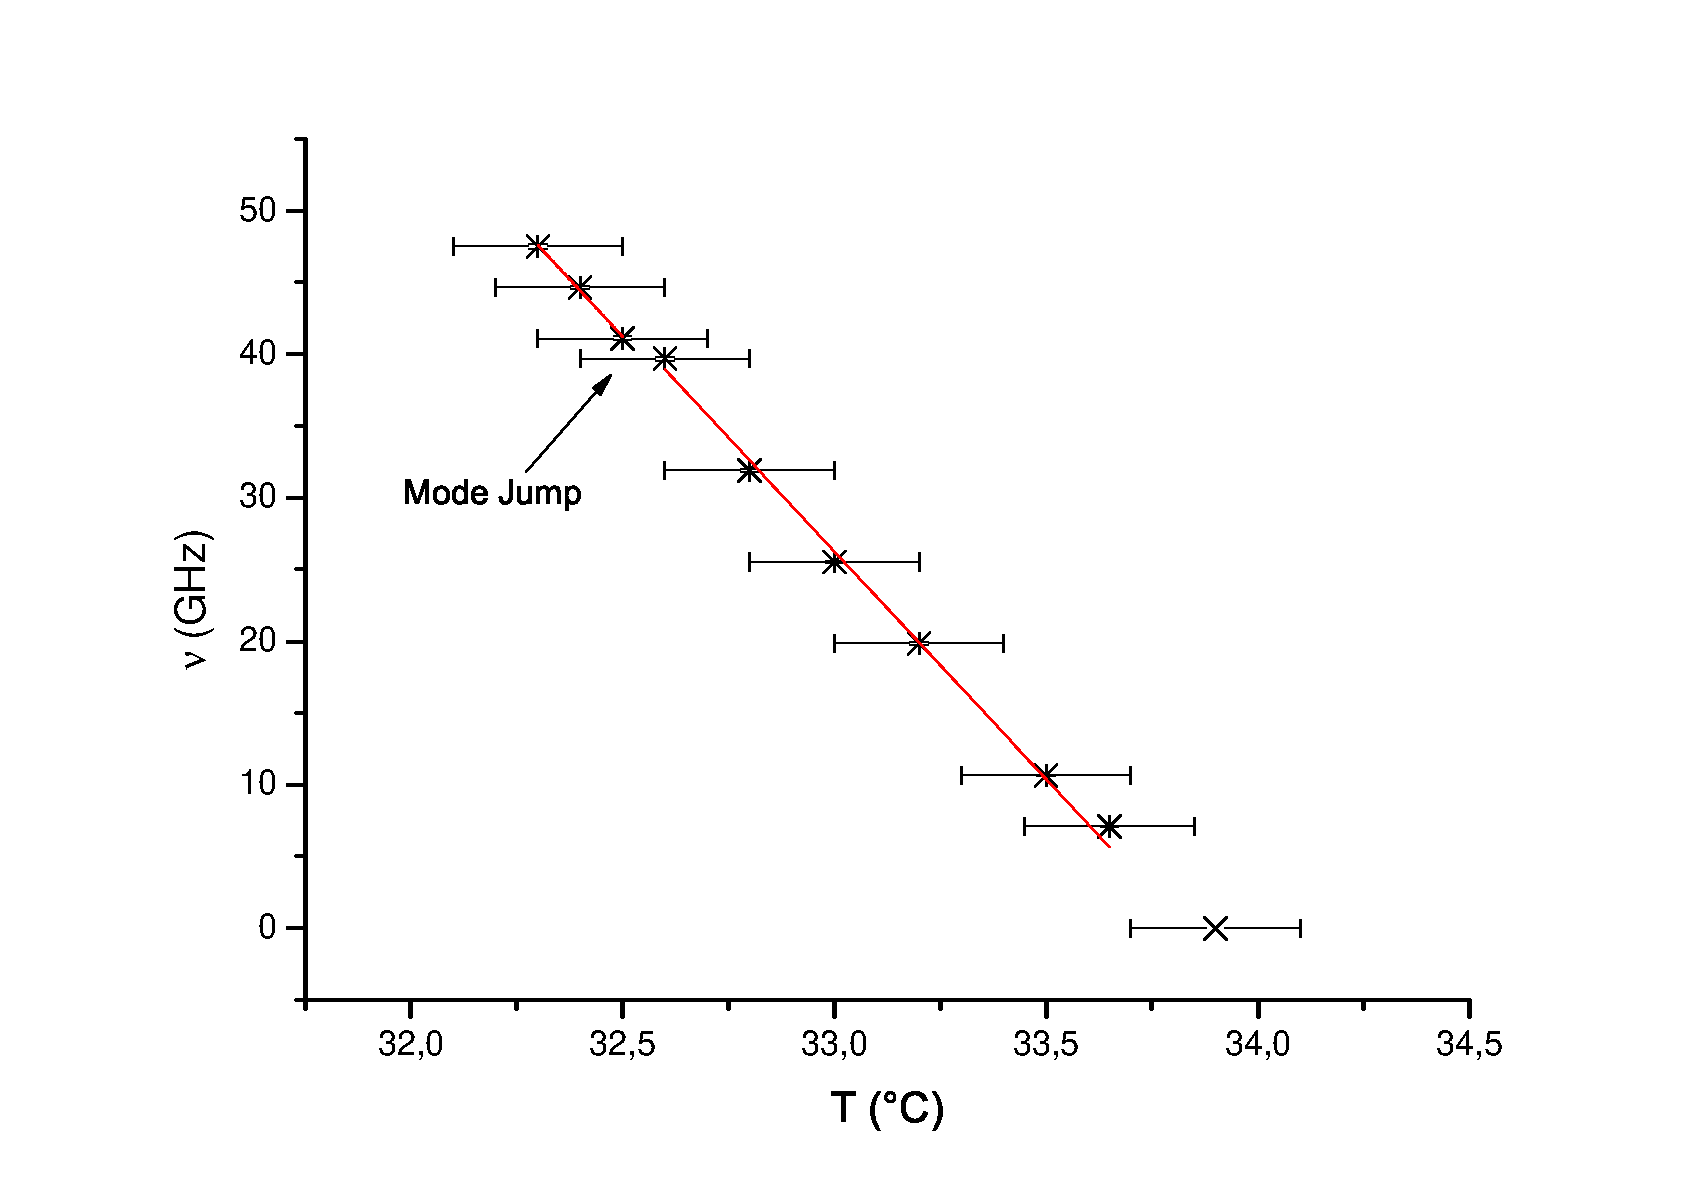
\includegraphics[width=0.9\textwidth]{BilderAusw/I_fest.pdf}
\caption{Variation of the laser temperature with constant current}
\end{figure}

Here, one is also able to see, that with increasing temperature, the frequency decreases. Also, we can see a mode jump near 32.5$^\circ C$. Both parts were fitted by a straight line, and the slopes are as follows:

\begin{center}
\begin{tabular}[H]{l l}
First Slope & $a_1 = (-31.81 \pm 2.05) \frac{GHz}{^\circ C}$\\
Second Slope & $a_2 = (-31.70 \pm 1.12) \frac{GHz}{^\circ C}$\\
\end{tabular}
\end{center}

For the rest of the measurements, we always used temperatures superior to 32,5 $^\circ C$, so the second slope is the one relevant as a conversion factor between temperature and frequency.

\subsubsection{Results}

\begin{tabular}[H]{l c}
Conversion Factors: & \\
Frequency-Current & $\Delta\nu = \Delta I \cdot (-3.858 \pm 0.056)\ {Ghz}/{mA}$\\
Frequency-Temperature & $\Delta\nu = \Delta T \cdot (-31.70 \pm 1.12)\ {Ghz}/{^\circ C}$\\
\end{tabular}


\subsection{Hyperfine Structure}

We installed the Rubidium cell into the optical path and removed the etalon. The laser diode was modulated by a triangular voltage with a peak-to-peak difference of $\sim 200\ mV$, and the temperature was set to $T = (34.6 \pm 0.2)^\circ C$, as described in the instructions. The preamplifier was set to AC from now on. However, with these adjustments we weren't able to find the hyperfine structure of the Rubidium atoms. Furthermore, the current of the laser diode wasn't able to surpass 35 mA and the preamplifier of the photodiode  was overcharged. We then tried different adjustments and installed a neutral filter (\emph{D 4,3}) into the optical path. The new adjustment was:\\

\begin{center}
\begin{tabular}[H]{l c}
Temperature & $T=34.4 ^\circ C$\\
Peak-to-Peak Voltage & $U_{pp} = 134\ mV$\\
\end{tabular}
\end{center}

We were then able to see the hyperfine structure at a current of $I = (62.9 \pm 0.3)\ mA$. With the same adjustments, we did another calibration. For this, however, we had to remove the filter, because the peaks weren't visible else. This measurement was also redone in the second week with the following adjustments:

\begin{center}
\begin{tabular}[H]{l c}
Temperature & $T=34.5 ^\circ C$\\
Peak-to-Peak Voltage & $U_{pp} = 4\ V$\\
Laser Current & $I = 63.9 mA$\\
\end{tabular}
\end{center}

\begin{figure}[H]
\centering 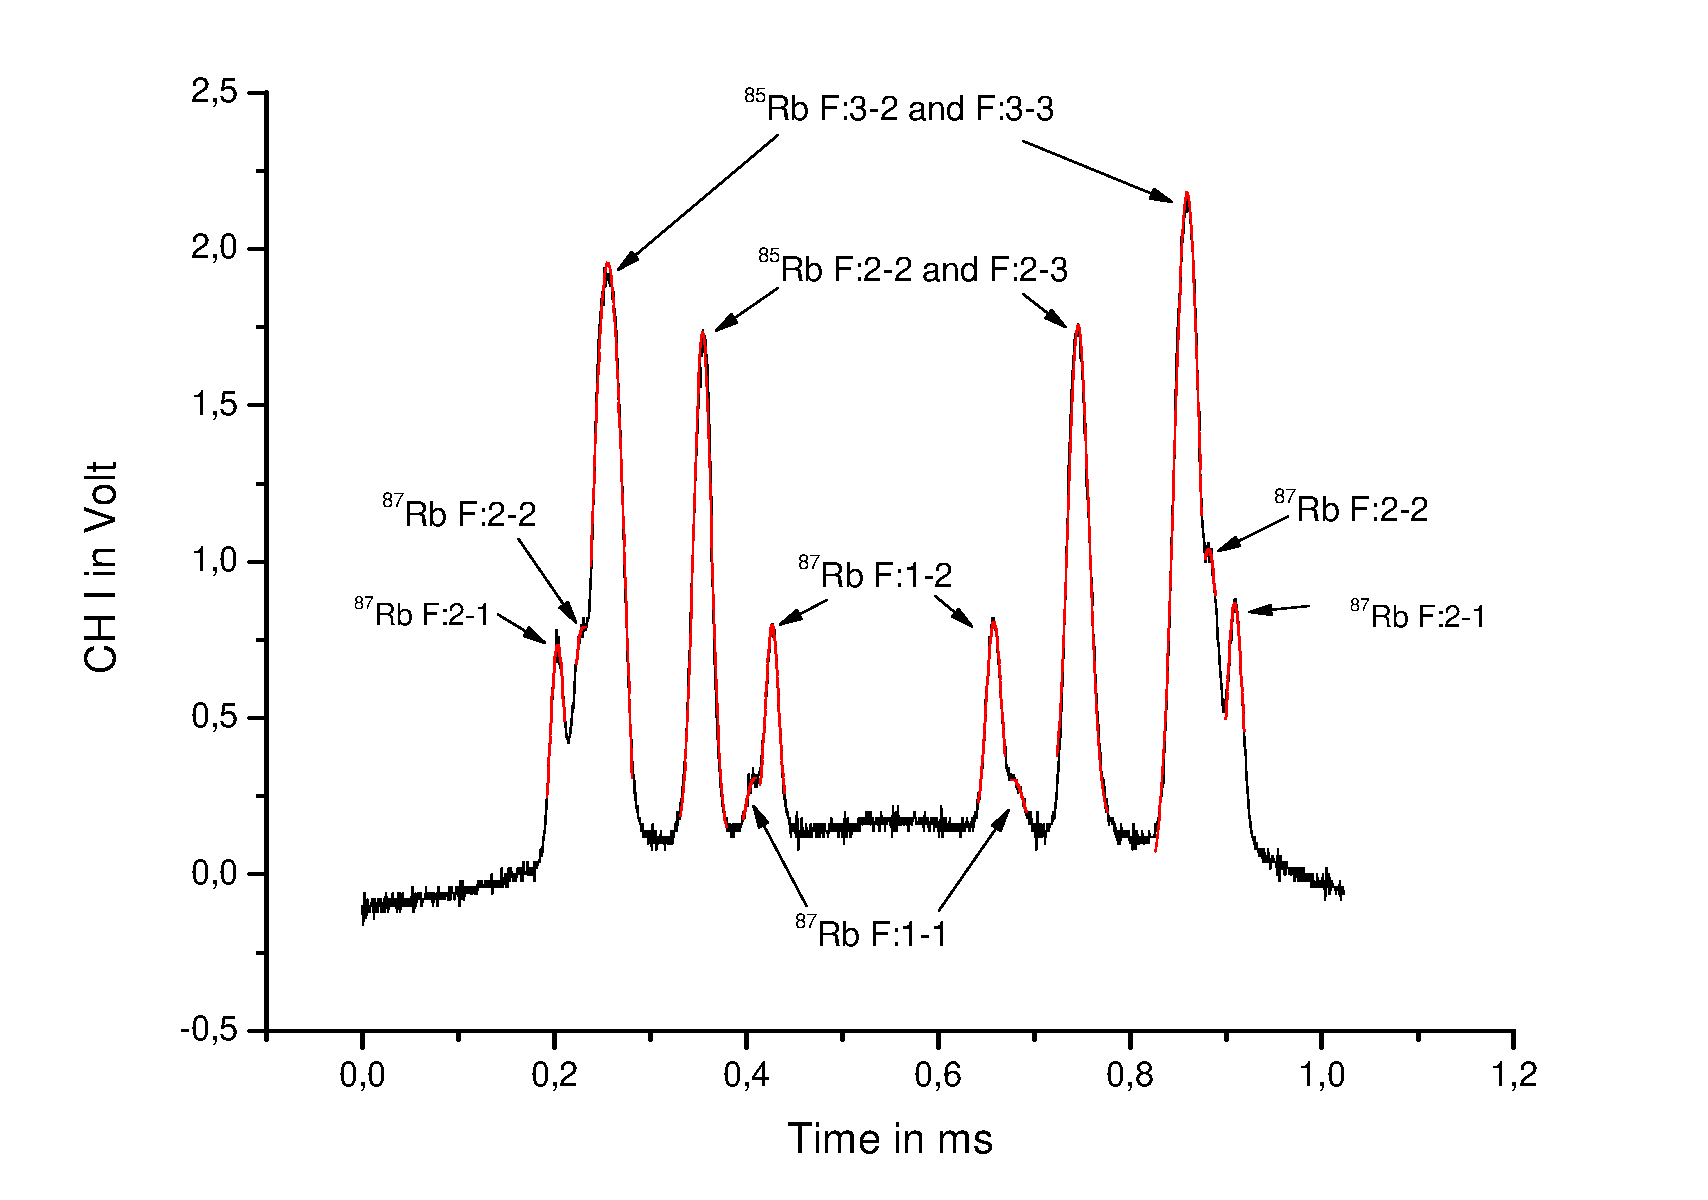
\includegraphics[width=0.96\textwidth]{BilderAusw/HFS.pdf}
\caption{Hyperfine spectrum of Rubidium}
\end{figure}

With the etalon, we were able to calibrate our measurements, i.e. to determine the time-frequency conversion factor $f$:

\begin{center}
\begin{tabular}[H]{l l}
Left side (descending laser current) & $f = (36.99 \pm 0.11) \frac{MHz}{\mu s}$\\
Right side (ascending laser current) &  $ f = (34.46 \pm 0.10) \frac{MHz}{\mu s}$\\ 
\end{tabular}
\end{center}

With this calibration and the position of the maxima, we can calculate their relative frequency. We assume the $^{85}Rb$ 3-2 and 3-3 peak to be known, so that we can determine the other peaks from the relative frequency in dependence of this one. The results are summarized in the following table:

\footnotetext[1]{Relative frequency to the $^{85}Rb$ 3-2 and 3-3 peak}



\begin{center}%--------- Kommastelle Fehler
\begin{tabular}[H]{| l | c c c c c |} \hline
 & Relative & error on & RF to the & RF$_{Theory}$ & Difference theory \\
Left Side & Frequency\footnotemark[1] (RF) & RF & D1-line & to D1 & experiment\\ \cline{2-6}
 & MHz & MHz & MHz & MHz & MHz \\ \hline \hline
1, $^{87}Rb$ F: 2-1 & -1934.4 & 77.7 & -3414.4 & -3070 & -344.4  	\\
2, $^{87}Rb$ F: 2-2 & -1320.4 & 65.4 & -2800.4 & -2250 & -550.4  	\\
3, $^{85}Rb$ F: 3-2(,3) &        0    & 0 & -1480 & -1480 & 0 		 \\
4, $^{85}Rb$ F: 2-2(,3) & 3650.5 & 120.5 & 2170.5 & 1560 & 610.5  		\\
5, $^{87}Rb$ F: 1-1 & 5662.6  & 176.3 & 4182.6 & 3760 & 422.6 		\\
6, $^{87}Rb$ F: 1-2 & 6328.3  & 195.3 & 4848.3 & 4580 & 268.3  		\\ \hline
\end{tabular}\\ 
\end{center}



\begin{center}%--------- Kommastelle Fehler
\begin{tabular}[H]{| l | c c c c c |} \hline
 & Relative & error on & RF to the & RF$_{Theory}$ & Difference theory \\
Right Side & Frequency\footnotemark[1] (RF) & RF & D1-line & to D1 & experiment\\ \cline{2-6}
 & MHz & MHz & MHz & MHz & MHz \\ \hline \hline
6, $^{87}Rb$ F: 1-2 & 6943.3 & 207.3 & 5463.3 & 4580 & 883.3 	\\
5, $^{87}Rb$ F: 1-1 & 6271.4 & 188.4 & 4791.4 & 3760 & 1031.4 	\\
4, $^{85}Rb$ F: 2-2(,3) & 3907.6 & 123.4 & 2427.6 & 1560 & 867.6 	\\
3, $^{85}Rb$ F: 3-2(,3) & 0 	  & 0 & -1480   & -1480 & 0  		\\
2, $^{87}Rb$ F: 2-2 & -765.0  & 53.5 & -2245.0& -2250 & 5.0  		\\
1, $^{87}Rb$ F: 2-1 & -1705.7& 69.5 & -3185.7& -3070 & -115.7 	\\ \hline
\end{tabular}
\end{center}

We estimate the error of the position (time) of a peak with about 1 ms. The error of the frequency is then given by:

$$s_\nu = \nu\cdot\sqrt{\left(\frac{s_t}{t}\right)^2 + \left(\frac{s_f}{f}\right)^2}$$

The error on the ''-1480-Peak'' is zero since it is set fixed.

\subsubsection{Determination of the interval constant}

The interval constant of the hyperfine structure is given by the formula:

$$ A = \frac{\Delta\nu\cdot h}{F+1} $$

whereas $\Delta\nu$ is the difference of the two frequencies for either the $^2S_{1/2}$ or $^2P_{1/2}$ state. The error is then given by:

$$ s_A = A\cdot\frac{s_{\Delta\nu}}{\Delta\nu} = A\cdot\frac{\sqrt{s_{\nu_1}^2 + s_{\nu_2}^2}}{\Delta\nu} $$

This leads to the following table:

\begin{center}
\begin{tabular}[H]{l | c c c}
Isotope & A in $10^{-6}$ eV & $A_{theoretical}$ in $10^{-6}$ eV & Standard deviations\\ \hline
$^{87}Rb$, $^2S_{1/2}$, left & $ 15.71 \pm 0.40 $ & 14.13 	& 4 	\\ %11-21
$^{87}Rb$, $^2S_{1/2}$, right & $ 16.50 \pm 0.41 $ & 14.13 	& 6	\\ %11-21
$^{87}Rb$, $^2P_{1/2}$, left & $1.38 \pm 0.54 $ & 1.692 		& 6	\\ %12 -11 
$^{87}Rb$, $^2P_{1/2}$, right & $ 1.39 \pm 0.58 $ & 1.692 	& 6	\\ %12-11
\end{tabular}\\
\end{center}

%------------------------------------------------

\clearpage
\subsection{Double Resonance}

For this part, we inserted the quarter-wave plate. We controlled its correct adjustment using a linear polarizer. Then, the radio frequency inductor coil (RF), situated on the Rubidium cell, was switched on. The current was set to about 10 V and the frequency was $\nu_{RF} = (499.3 \pm 0.3) kHz$, which we measured with a frequency counter. We then tried to find the correct adjustments for the laser diode. We did this by modulating the inductor coil 2 with a sawtooth function with a large amplitude and then varying the laser current until absorptions were visible. Having found the correct laser current, we changed the sawtooth function to a sine modulation in order to start the measurements.

With the sawtooth, we found the following laser currents to show absorption lines in the spectrum:

$$ I_1 = (65.4 \pm 0.2)\ mA $$
$$ I_2 = (64.9 \pm 0.2 )\ mA $$

The temperature of the laser diode was $T=(34.0 \pm 0.2)^\circ C$
 
\begin{figure}[H] 
\begin{minipage}{0.5\textwidth} 
\centering 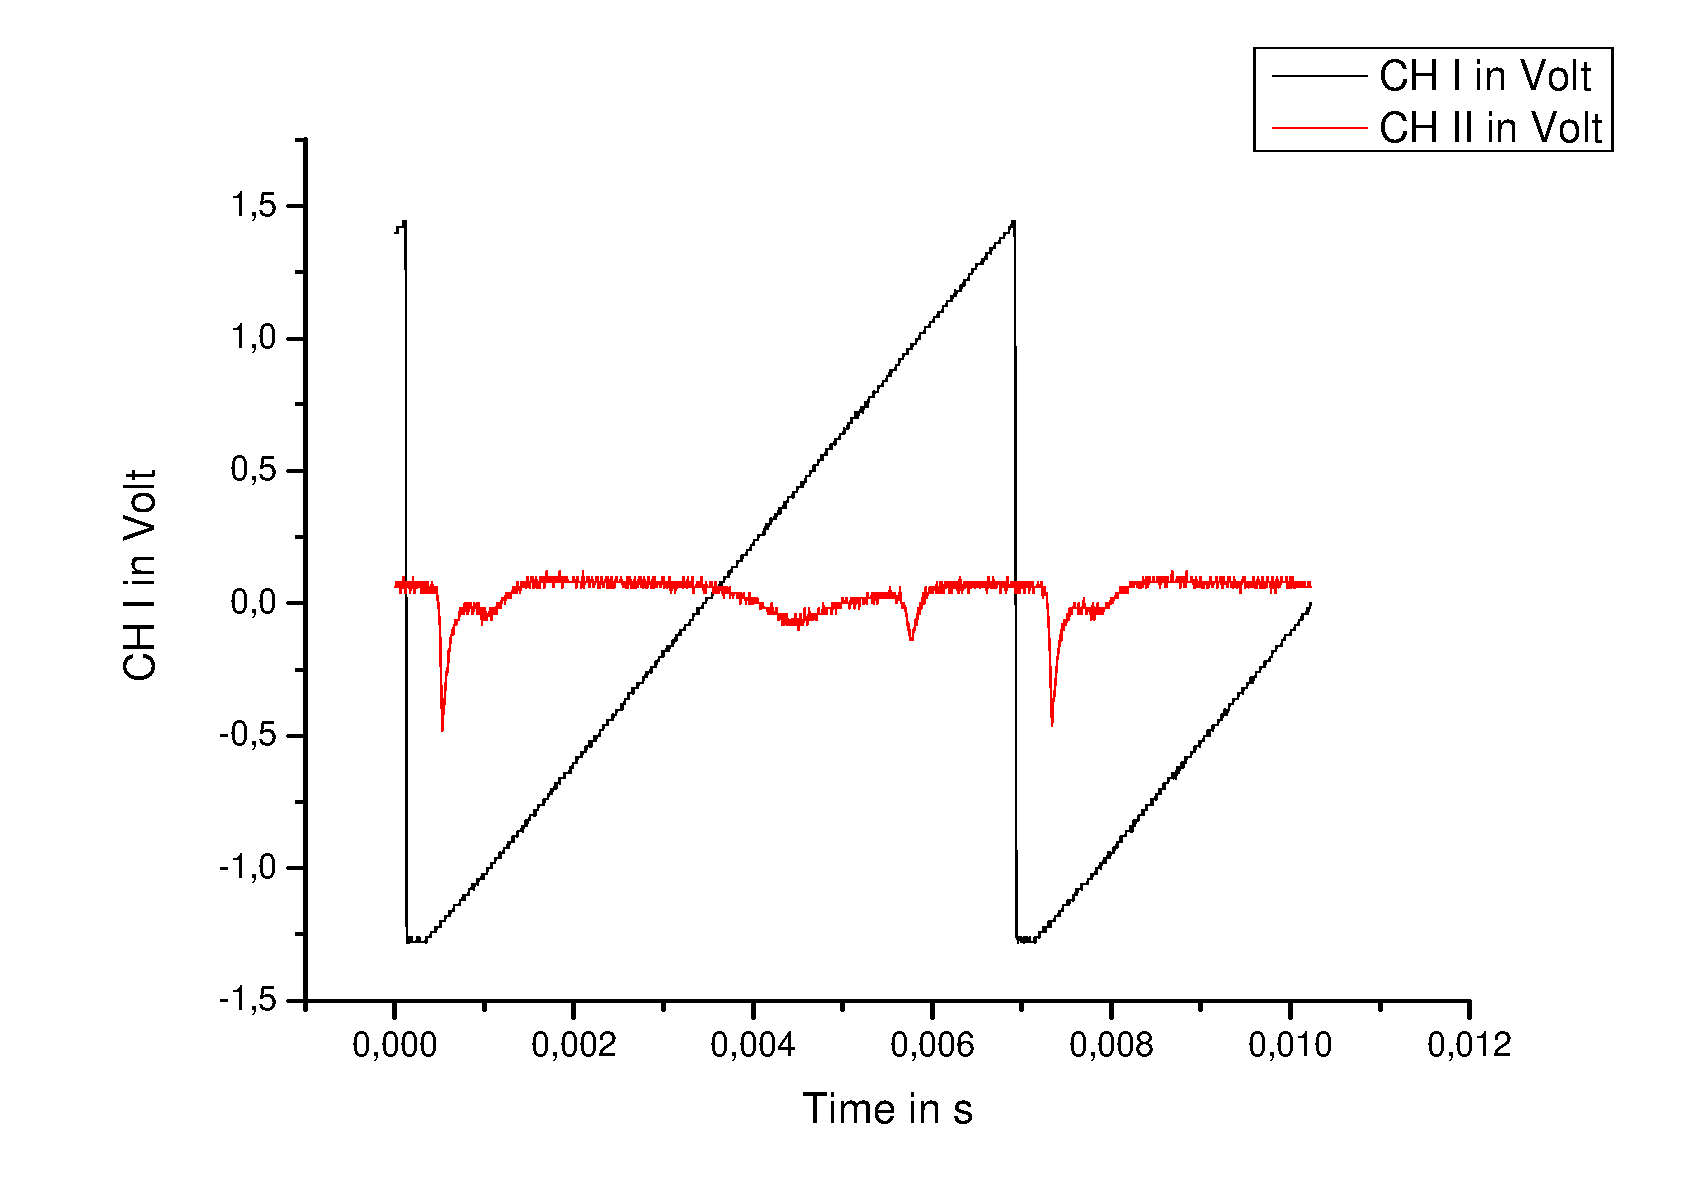
\includegraphics[width=\textwidth]{BilderAusw/DR_1.pdf}
\caption{Absorption at $I = 64.9\ mA$}
\end{minipage}
\begin{minipage}{0.5\textwidth} 
\centering 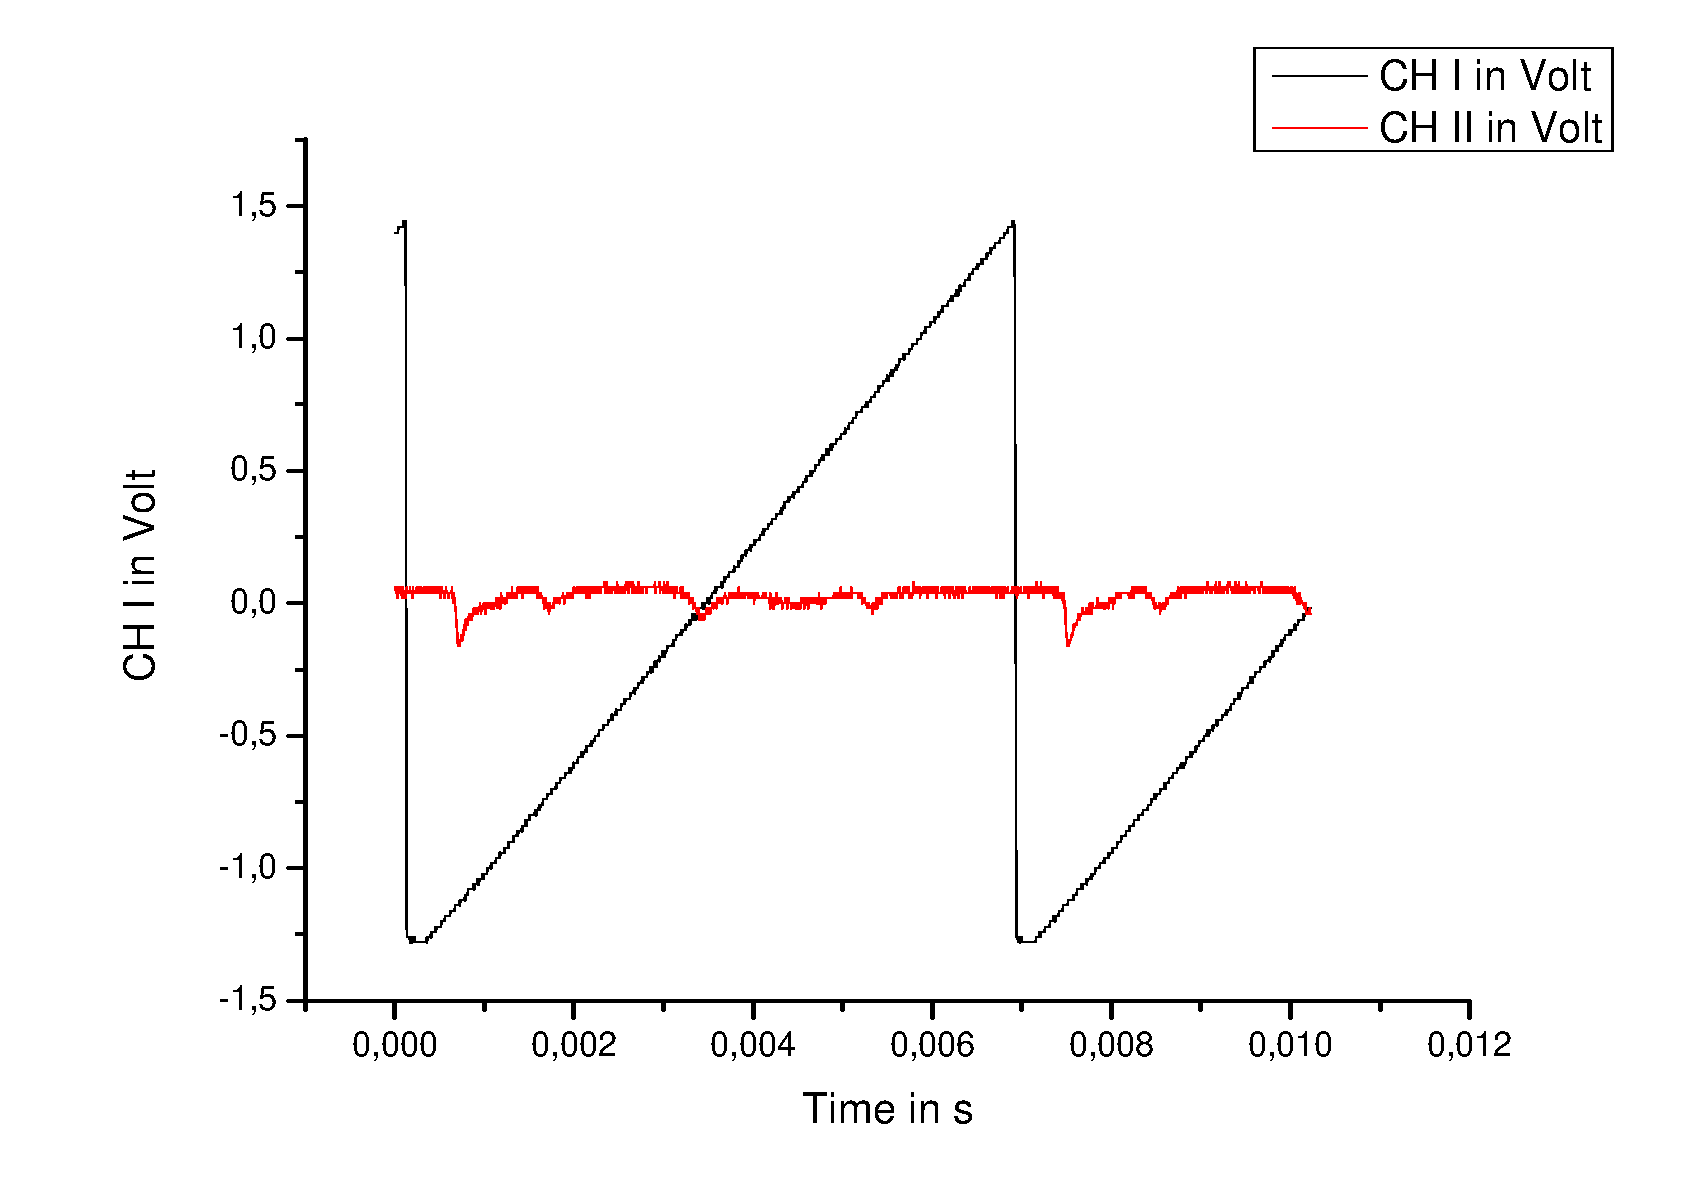
\includegraphics[width=\textwidth]{BilderAusw/DR_2.pdf}
\caption{Absorption at $I = 65.4\ mA$}
\end{minipage}
\end{figure}

The inductor coil 2 was then modulated with a sine function of 50 Hz and the laser was set to one of the two resonance frequencies. The current through the inductor coil 1 was then changed until the visible absorption peaks were equidistant and then the current of the inductor coil 4 was changed in order to make the peaks as high as possible. After the adjustment of the coil 4, we readjusted the coil 1, to assure equidistance of the peaks. Then the polarity of inductor coil 1 was reversed and the equidistance was readjusted. We got the following values:

\begin{center}
\begin{tabular}[H]{c | c c c}
Resonance Current & $I(coil1)/mA$ & $I(coil1)_{rev.pol.}$ & $I(coil4)/mA$ \\ \hline
$I_1 = (65.4 \pm 0.2)\ mA$ & $102 \pm 1$ & $79 \pm 1$ & $80 \pm 5$ \\
$I_2 = (64.9 \pm 0.2 )\ mA$ & $144 \pm 1$ & $123\pm1$ & $84\pm5$ \\
\end{tabular}
\end{center}

These values allow us to determine the earth's magnetic field. The magnetic field of the induction coil 4 cancels the vertical magnetic field of the earth, which means, that it should have the same value. The difference between the two magnetic fields of both polarities should be twice the earth's horizontal magnetic field.\\

\begin{figure}[H]
\centering 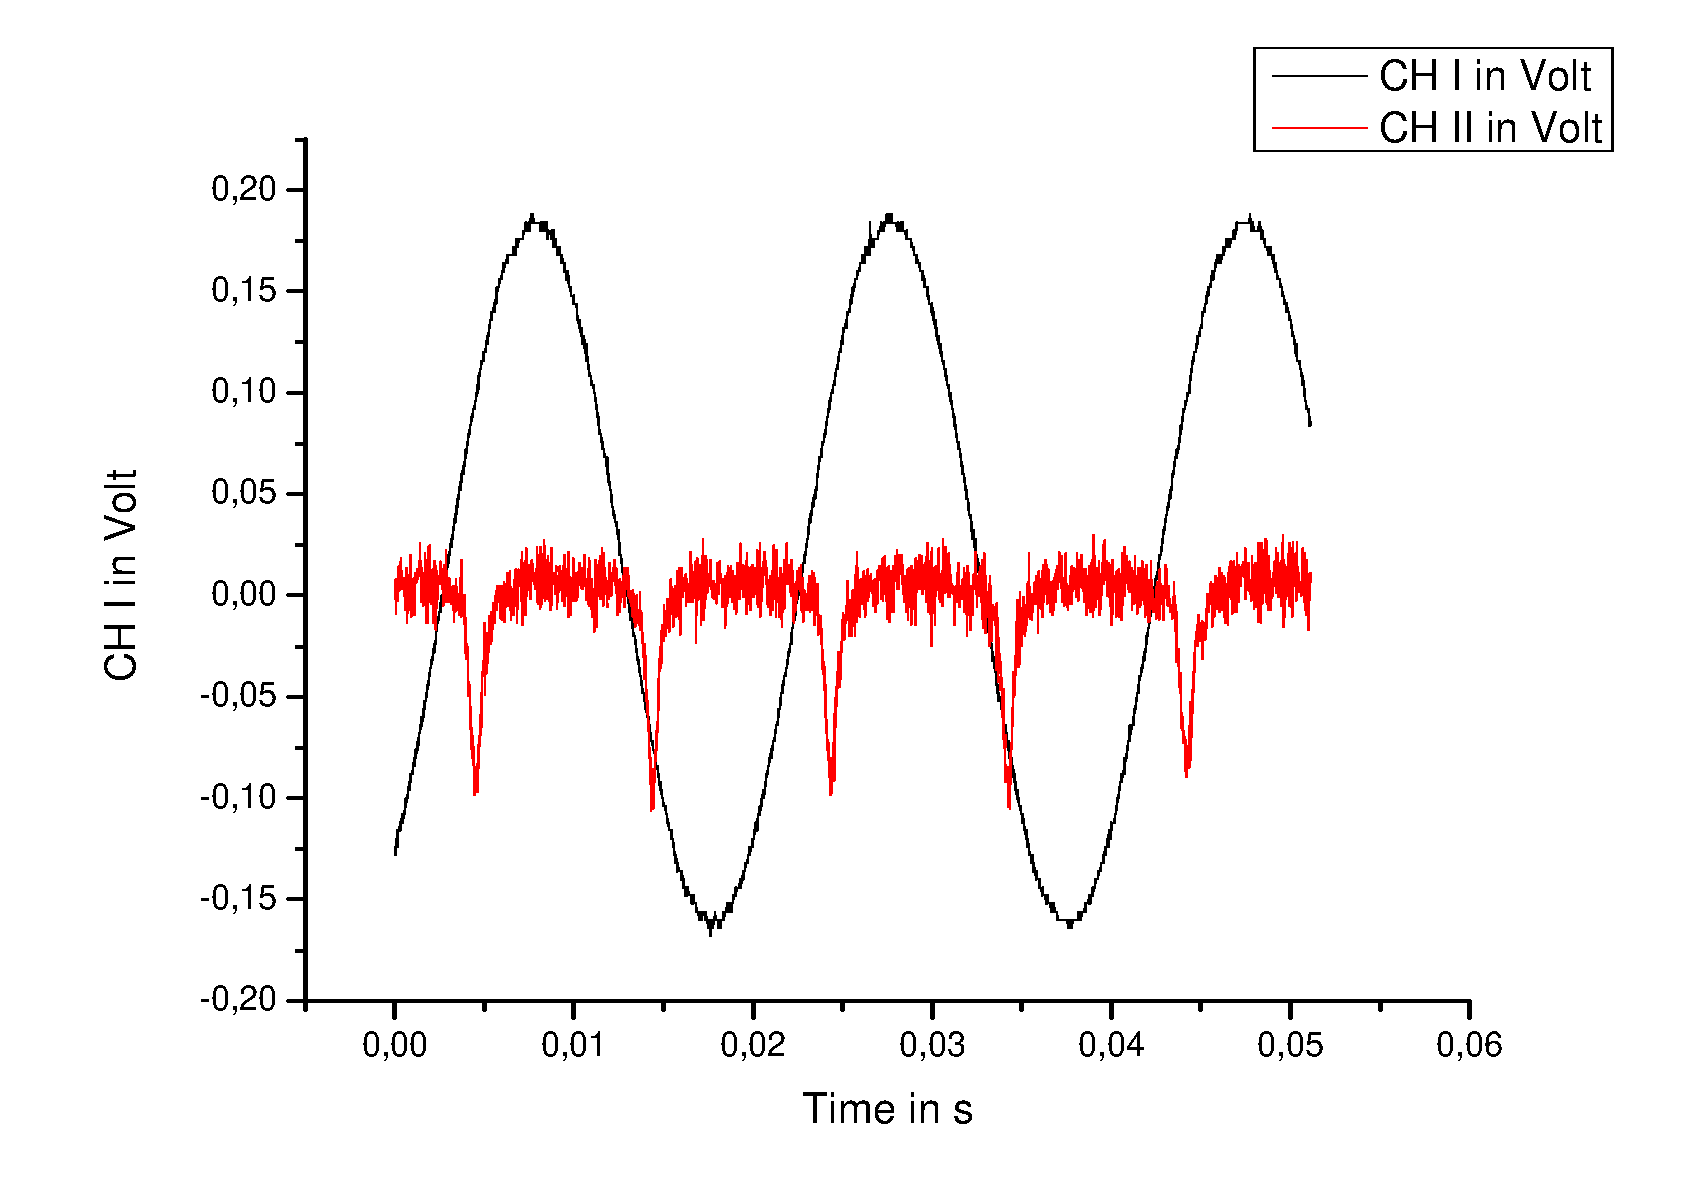
\includegraphics[width=0.75\textwidth]{BilderAusw/DRequi.pdf}
\caption{Equidistant Absorption Peaks}
\end{figure}


To calculate the magnetic field from the current through the coils, we use the measured values given in the experiment's description:

\begin{figure}[H]
\centering 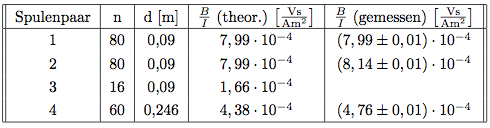
\includegraphics[width=0.75\textwidth]{BilderAusw/Spulenumr.png}
\end{figure}

So, $B=a\cdot I$ whereas $a$ is the conversion factor. Since for coil 1: \ $I=\frac{1}{2}|I_{pol1}-I_{pol2}|$, the error is $$s_I^{coil1} = \sqrt{s_{I_{pol1}}^2 + s_{I_{pol2}}^2} = 1.41$$
The error for B is then:

$$s_B = B\cdot\sqrt{\left(\frac{s_a}{a}\right)^2 + \left(\frac{s_I}{I}\right)^2}$$

We calculate the following values:

\begin{center}
\begin{tabular}[H]{c | c c}
 & Horizontal magnetic field & Vertical magnetic field \\ \hline
Current $I_1$ & $B_{hor}^{(1)} = (9.19 \pm 1.1)\ \mu T$ & $B_{vert}^{(1)} = (38.08 \pm 2.38)\ \mu T$\\
Current $I_2$& $B_{hor}^{(2)} = (8.39 \pm 1.1)\ \mu T$ & $B_{vert}^{(2)} = (39.98 \pm 2.38)\ \mu T$\\
Theoretical Values & $B_{hor} = 20.9 \mu T$ & $B_{vert} = 42.9 \mu T$\\
Standard Deviations & 11, 12 & 3, 2\\
\end{tabular}
\end{center}

As one can see, the values for the horizontal field clearly differ from the theoretical values ($\sim$ factor 2). Since the theoretical horizontal value is meant to be the magnetic field in north-south direction, it occurred to us that maybe the optical bench didn't point in that specific direction. We used a compass to realign the table, so that the photo diode pointed towards north and the laser diode was south from it. The table now had an angle of about 30$^\circ$ towards its initial position. By using the compass, we detected that the optical bench itself was magnetized, which we assumed to be a potential disturbance source.

\begin{figure}[H]
\centering 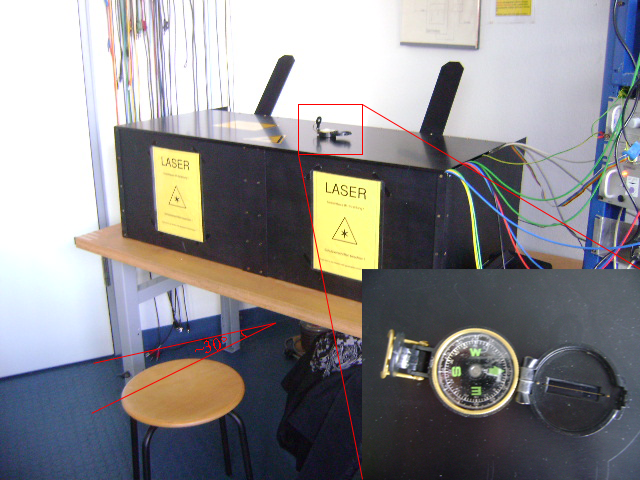
\includegraphics[width=\textwidth]{BilderAusw/Nordsued.png}
\caption{North-South orientation of the optical bench}
\end{figure}

With this new orientation, we redid all the measurements from scratch. The results are summarized in the following tables. (Laser temperature : $T=(34.1 \pm 0.2)^\circ C$)

\begin{center}
\begin{tabular}[H]{c | c c c c c}
 & $I(pol1)_{coil1}/mA$ & $I(pol2)_{coil1}/mA$ & $I_{colt4}/mA$ & $B_{hor}/\mu T$ & $B_{vert}/\mu T$\\ \hline
$I_{Laser} = (65.3 \pm 0.2)$ & $105 \pm 1$ & $74 \pm 1$ & $ 81\pm 5$ & $12.38 \pm 1.13$ & $38.56 \pm 2.38$\\
$I_{Laser} = (64.9 \pm 0.2)$ & $151 \pm 1$ & $120 \pm 1$ & $ 83\pm 5$ & $12.38 \pm 1.13$ & $39.51 \pm 2.38$\\
\end{tabular}
\end{center}

The theoretical value for the horizontal field lies within the 8th standard deviation of both our calculated values and the theoretical value of the vertical field lies within the 2nd. The value for the horizontal field greatly improved, the one for the vertical field slightly improved too. We can assume, as discussed before, that the fact that our values lie underneath the theoretical value, is due to the magnetization of the optical bench. Also, the abrasion of the induction colts could be a potential error source.

\subsubsection{The nuclear spin}

We determine the nuclear spin of the Rubidium isotopes with the formula:

$$ I = \frac{\mu_BB}{h\nu_{RF}}-\frac{1}{2} $$

The vertical magnetic field was compensated by the induction colt 4. $B$ is the magnetic field of colt 1 when the peaks are equidistant subtracted by (resp. added to) the earth's horizontal magnetic field. $\mu_B$ is the Bohr magneton.

The error of the nuclear spin is determined by:

$$ s_I = I\cdot\sqrt{\left(\frac{s_B}{B}\right)^2 + \left(\frac{s_{\nu_{RF}}}{\nu_{RF}}\right)^2} $$

We have

$$I_1 = (84.5 \pm 1.5) mA \Rightarrow B_1 = (67.52 \pm 1.20)\mu T$$
$$I_2 = (130.5 \pm 1.5) mA \Rightarrow B_2 = (104.27 \pm 1.21)\mu T$$

The nuclear spins are:

\begin{center}
\begin{tabular}[H]{| l c c c c |}\hline
Isotope & Nuclear Spin & Theoretical Value & Error & Standard Deviations \\ \hline
(1)\ \ $^{87}Rb$ & $1.39 \pm 0.02$ & 1.5 & 7.3\% & 6 \\
(2)\ \ $^{85}Rb$ & $2.42 \pm 0.01$ & 2.5 & 3.2\% & 8\\  \hline
\end{tabular}
\end{center}

The measured values lie close to the theoretical ones. The error on the value is very small, so that a systematical error seems to cause most of the deviation. Again, the disturbing fields, such as the magnetization of the optical bench and other magnetic fields seem to have a non-negligible effect on the experiment and lead to this error.

%------------------------------------------------

\clearpage
\subsection{Spin Precession}

Firstly, we compensated the horizontal field with the induction coil 1, i.e. we set it to 15.5 mA (we adjusted it in a way that the ampere meter flickered between 15 and 16 mA since it doesn't have more digits). The coil 4 and the RF were turned off.

We then modulated the current of the induction coil 5 with a rectangular function and adjusted the offset, so that the minima of the rectangular function lie on 0. This periodically turns on and off the magnetic field, so that the atoms are aligned by the magnetic field and then suddenly the field ceases. The result is, that the atoms' angular momentum precesses around the earth's vertical magnetic field the moment the field is turned off and by measuring the frequency $\nu_{osz}$ of this precession, we can measure the earth's magnetic field using the formula:

$$ B_{vert} = \frac{h}{g_F\mu B}\nu_{osz} $$

We made 4 different measurements of this precession around the earth's vertical magnetic field. A measurement looks like this:

\begin{figure}[H]
\centering 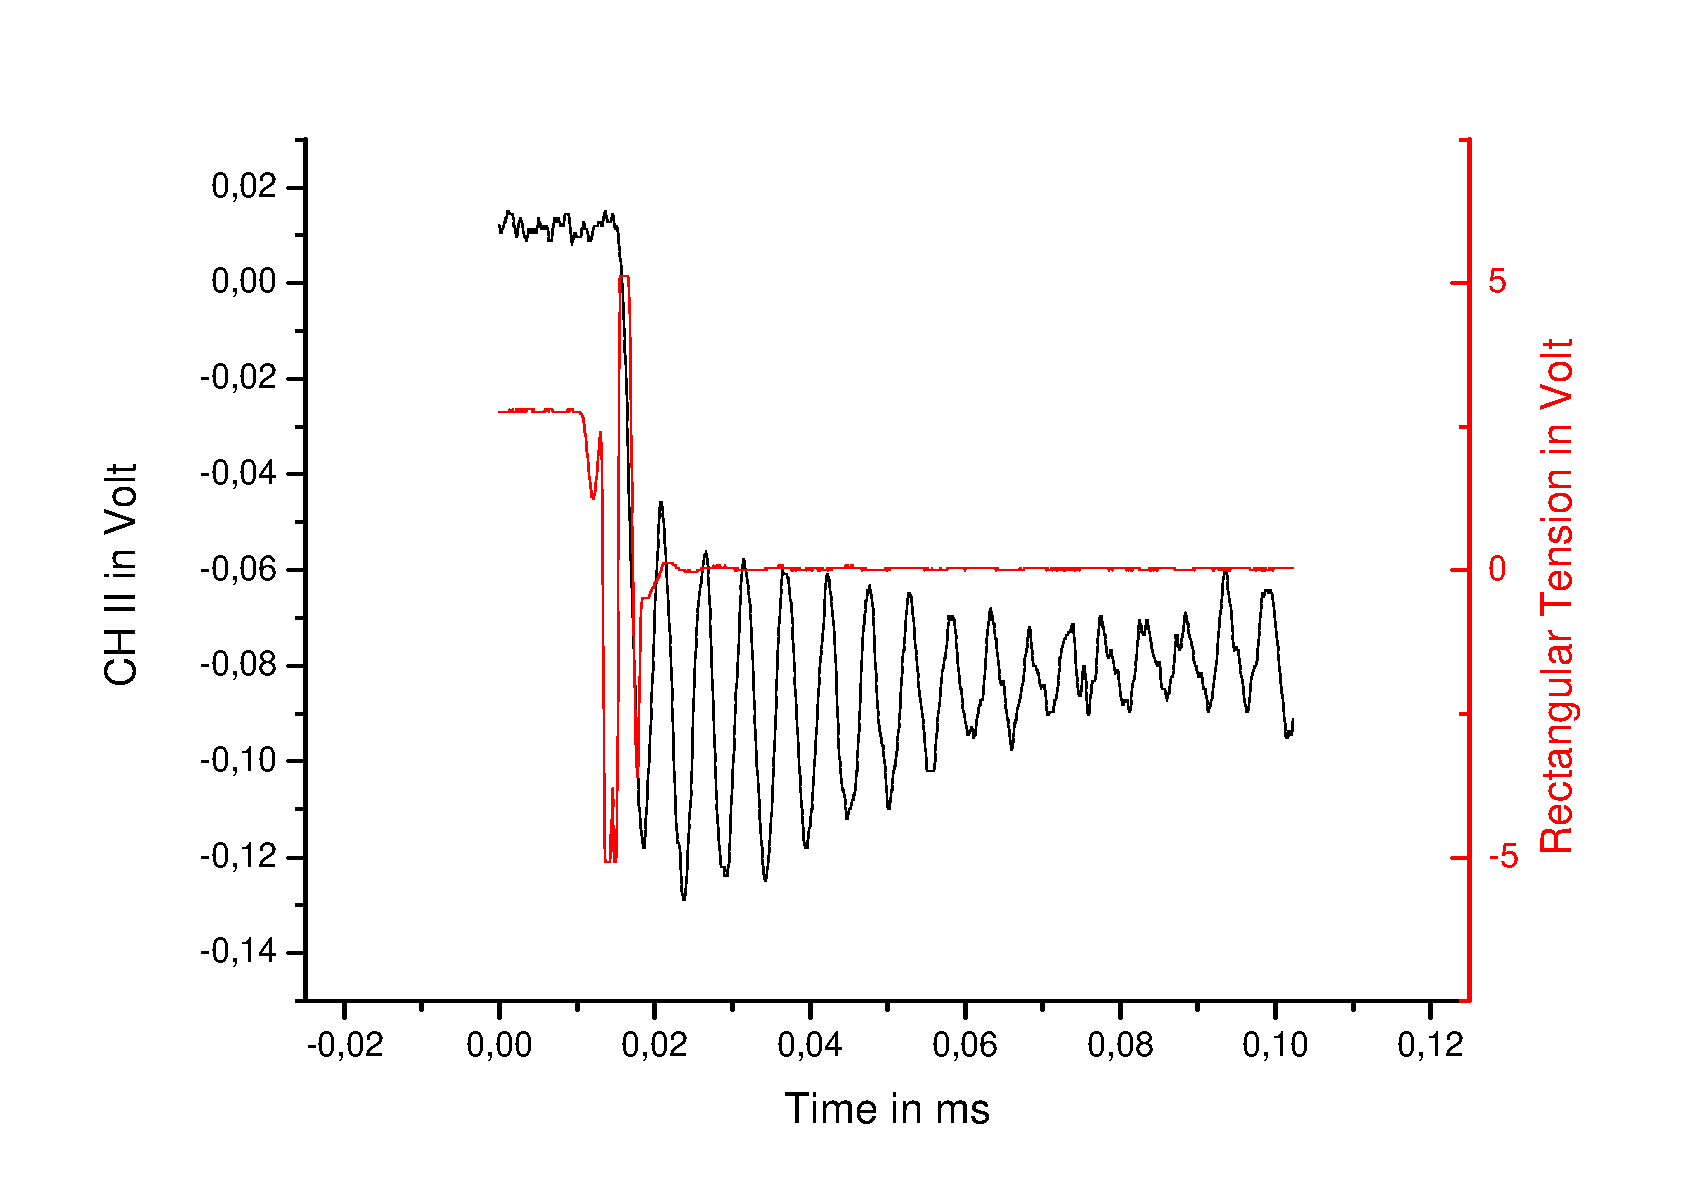
\includegraphics[width=\textwidth]{BilderAusw/Spinpr.pdf}
\caption{Spin precession around the earth's vertical magnetic field}
\end{figure}

As one can see, the rectangular function made a bit of a jump at the edges. This led to a lot of trouble getting clear sine waves. We had to strongly average the signal in order to actually be able to see the desired signal.

Our measurements are: ($s_t = 0.2 \mu s \Rightarrow s_{\Delta t} = 0.28 \mu s$)

\begin{center}
\begin{tabular}[H]{c c c}
$\Delta t$ & \# Periods & $T/\mu s$\\ \hline
42.35 & 8 & $5.294 \pm 0.035$\\
20.9   & 4 & $5.225 \pm 0.071$\\
37.0   & 7 & $5.286 \pm  0.040$\\
31.6   & 6 & $5.267 \pm  0.047$\\
\end{tabular}
\end{center}

This leads to a weighted average of

$$ \bar T = (5.279 \pm 0.022)\ \mu s \ \ \ \Rightarrow \ \ \ \nu_{osz}=\frac{1}{\bar T}= (189.44 \pm 0.79)\ kHz$$

Finally, we can calculate the earth's vertical magnetic field using the formula mentioned above and using $g_F = 1/3$\footnote{The measurement was done for the $^{85}Rb$-Isotope in the ground state} and find:

$$\boxed{ B_{vert} = (40.60 \pm 0.17)\ \mu T }$$\\

Compared to the theoretical value of $42.9\ \mu T$, we find a value which lies very close to it, i.e. we have a deviation of $\sim 5\%$, respectively 14 standard deviations. Again, the previously described systematical errors also take place.

If we change the current through the induction coil 4, i.e. its magnetic field, we get a different oscillation frequency with the same measurement. This is because the magnetic field of the coil 4 adds itself to the earth's vertical magnetic field, and the precession happens around the resulting field (which can be larger or smaller, depending on the polarization of the coil).  We measured this for about 25 different currents through the coil 4. The results are summarized in the graph below. The negative values represent the magnetic field in the opposite direction than the earth's field, and the positive values in the same direction.\\

The relation between the oscillation frequency and the magnetic field is given by the equation

$$\nu_{osz} = bx + a = (4.78\pm0.04)B_{vert} + (187.52\pm1.13)$$

Here the intercept leads to

$$B_{vert} = (40.18 \pm 0.24)\mu T$$

respectively, one can calculate the compentsating field of the coil 4 by setting the frequency to zero, i.e. calculating the intercept at the x-axis. This means:

$$ y = bx + a = 0 \Leftrightarrow x = \frac{-a}{b} = -39.19 \mu T $$

Considering the error, this leads to a value of:

$$ B_{vert} = (39.19 \pm 0.01)\ \mu T $$

Both values lie pretty close to the theoretical value. The error of the latter one is not representative.

\begin{figure}[H]
\centering 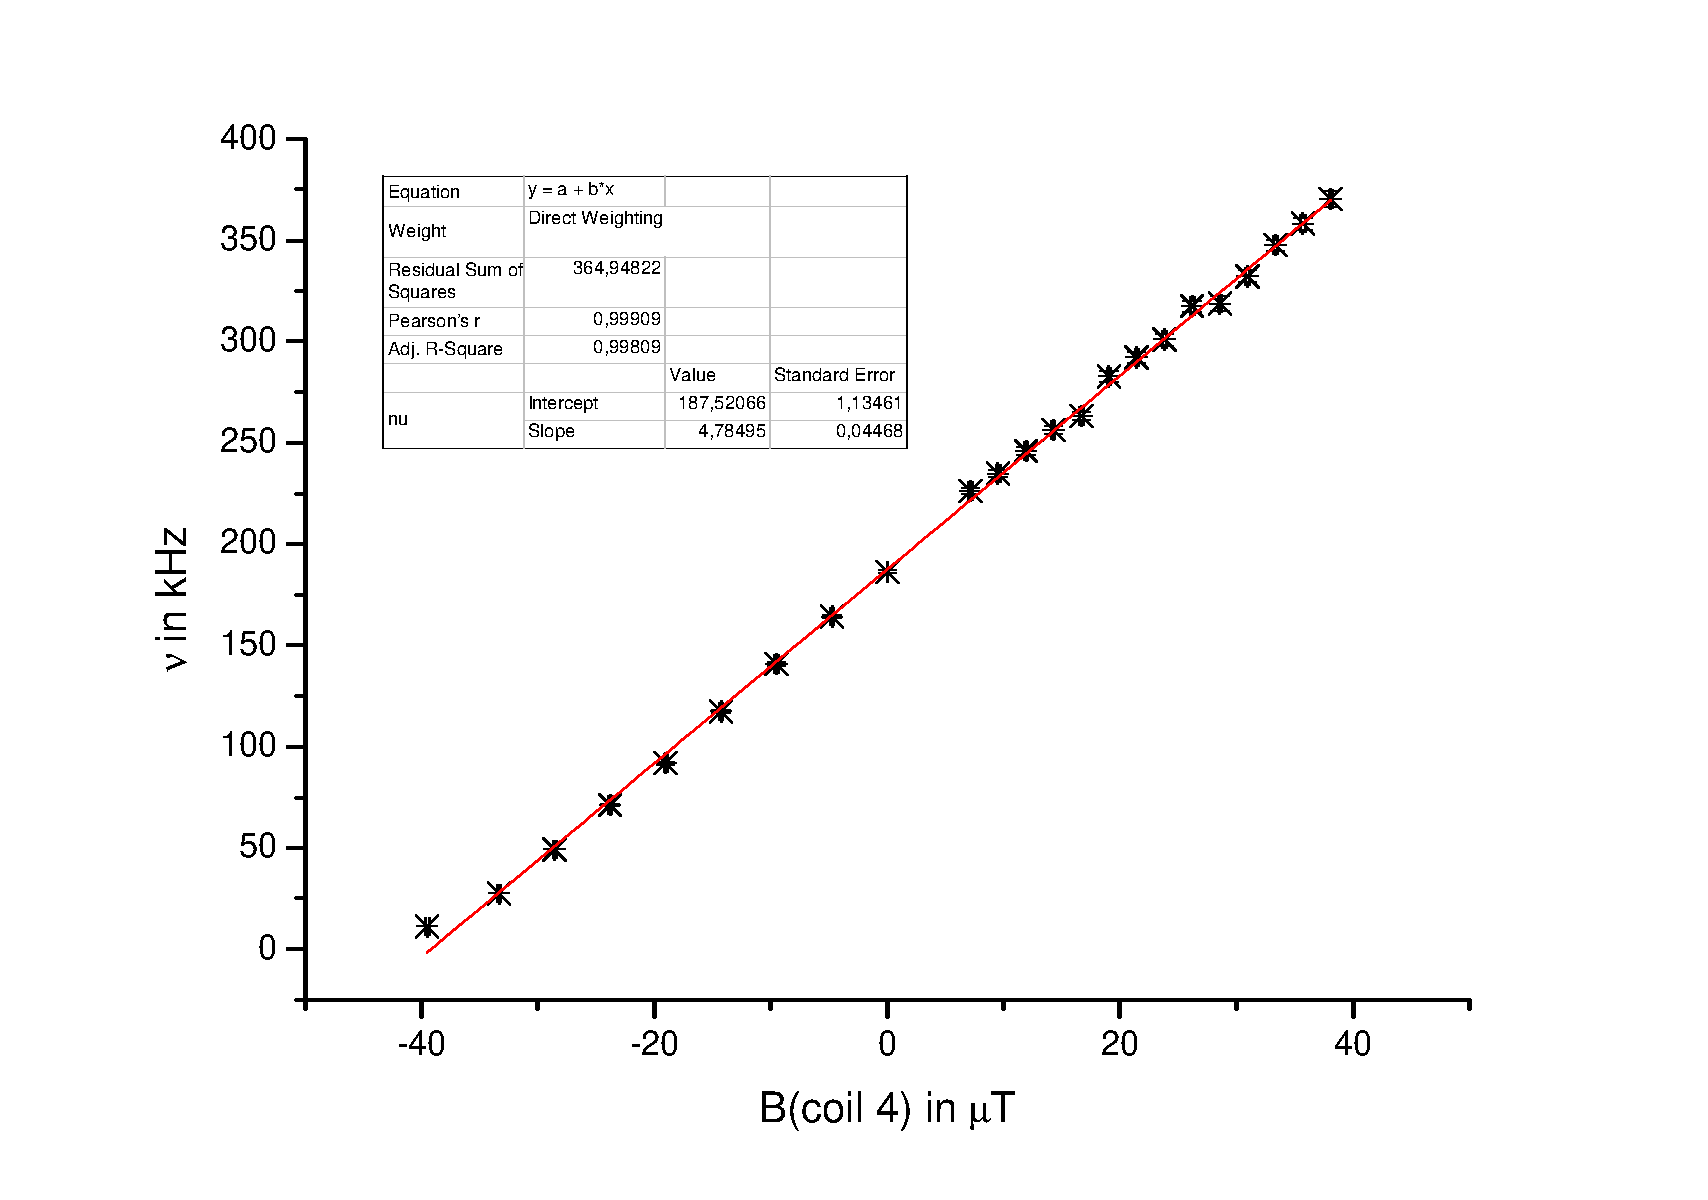
\includegraphics[width=1.1\textwidth]{BilderAusw/praezfeld.pdf}
\caption{Spin precession around the resulting vertical magnetic field}
\end{figure}

%------------------------------------------------

\subsection{Relaxation Time (Dehmelt)}

For the measurement of the relaxation time according to Dehmelt, we turn off the induction coil 1 and use the coil 4 to compensate the earth's vertical magnetic field ($I(coil4) = 83\ mA$). The induction coil 3 was modulated with a rectangular tension, whose purpose was to reverse orientation of the magnetic field periodically. After the reorientation, the Rubidium atoms took a certain time to be pumped back into the state of maximal polarization; this time is the relaxation time we want to find out. The temperature was set to 34.3$^\circ C$.\\

We tried first measurements, but weren't able to see any good absorptions. We then had the idea to constantly heat the Rubidium cell in order to see more, using a hair dryer. The problem is, that the relaxation time depends on the pressure in the Rubidium cell, so we had to keep the cell at the same temperature for all the measurements, i.e. we constantly blow-dryed the cell.\\

We then measured the absorption lines for 8 different normal filters. The filters themselves were measured using a voltmeter (\emph{ELTELEC DM 101}) and comparing the tension on the photo diode to the tension without the filter.\\

We found the following data:

\begin{center}
\begin{tabular}[H]{l | c c}
Filter & $U in mV$ & $U/U_0$ \\ \hline
none & $597 \pm 12$ &    $1$\\
D0,6 & $223 \pm 5$ &        $0.374 \pm 0.010$ \\
D1,0 & $111.5 \pm 2.2$ & $ 0.187 \pm 0.005$ \\
D2,0 & $42.2 \pm 0.8$ &   $ 0.071 \pm 0.002$\\
D2,3 & $29.5 \pm 0.6$ &   $ 0.049 \pm 0.001$\\
D2,6 & $22.5 \pm 0.5$ &    $0.038 \pm 0.001$\\
-0,8  & $114.3 \pm 2.3$ &  $0.191 \pm 0.005$\\
-1,03 & $66.8 \pm 1.3 $&   $0.112 \pm 0.003$\\
-1,24 & $48.1 \pm 1.0$ &   $0.081 \pm 0.002$\\
\end{tabular}
\end{center}

An absorption line looks as following: 

\begin{figure}[H]
\centering 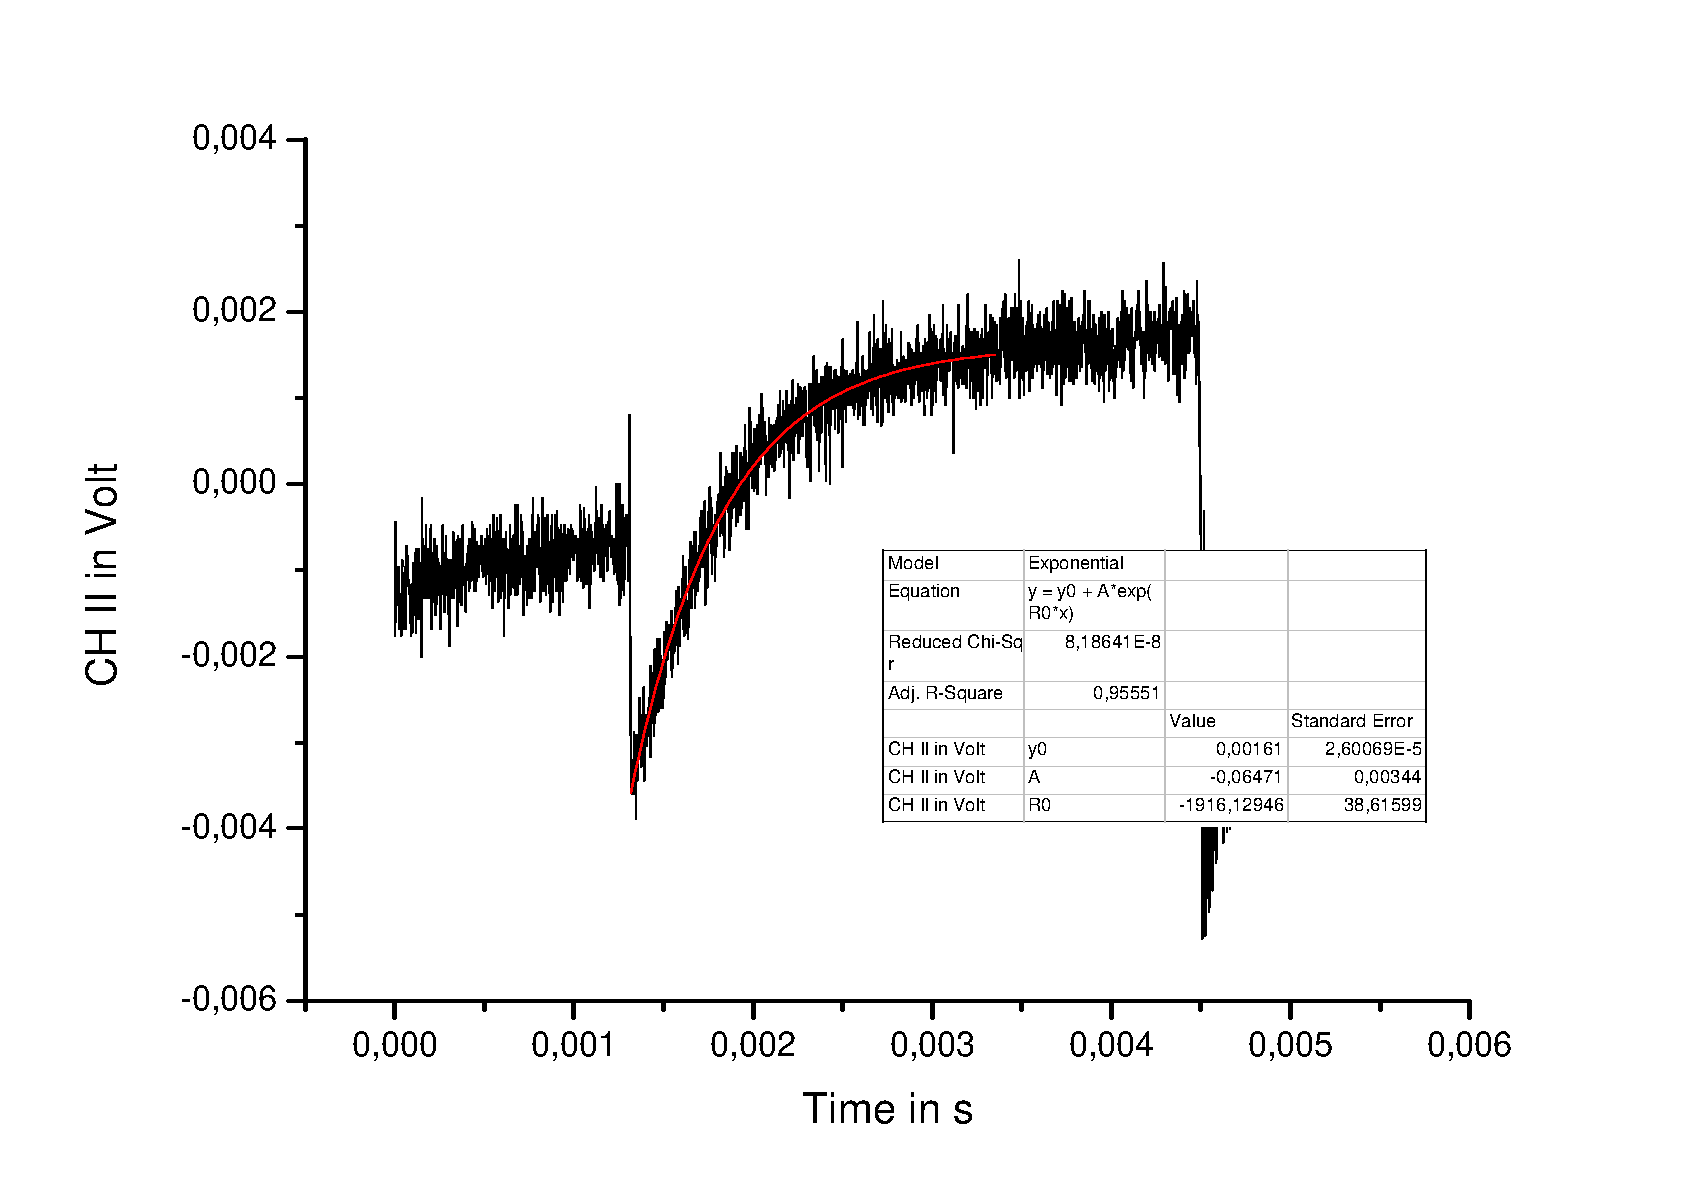
\includegraphics[width=0.95\textwidth]{BilderAusw/DehmeltBsp.pdf}
\caption{Example of an absorption line}
\label{dehmeltbsp}
\end{figure}

We fitted the curve with an exponential function $y=y_0 + A\exp(R_0\cdot x)$, with $R_0 = -1/\tau$, where $\tau$ is the orientation time. We then plotted $\tau^{-1}$ against $U/U_0$ and fitted the curve by with a straight line. The intercept at the y-axis should then exactly be the sought relaxation time $T_R$. This is, because

$$\frac{1}{\tau} = \frac{1}{T_R} + \frac{1}{T_P}$$

and $T_P \sim I^{-1}$ is the pumping time. So if $I \to 0$, then we have $\frac{1}{T_P} = 0$ and then $\tau = T_R$. Our plot looks like this:\\

\begin{figure}[H]
\centering 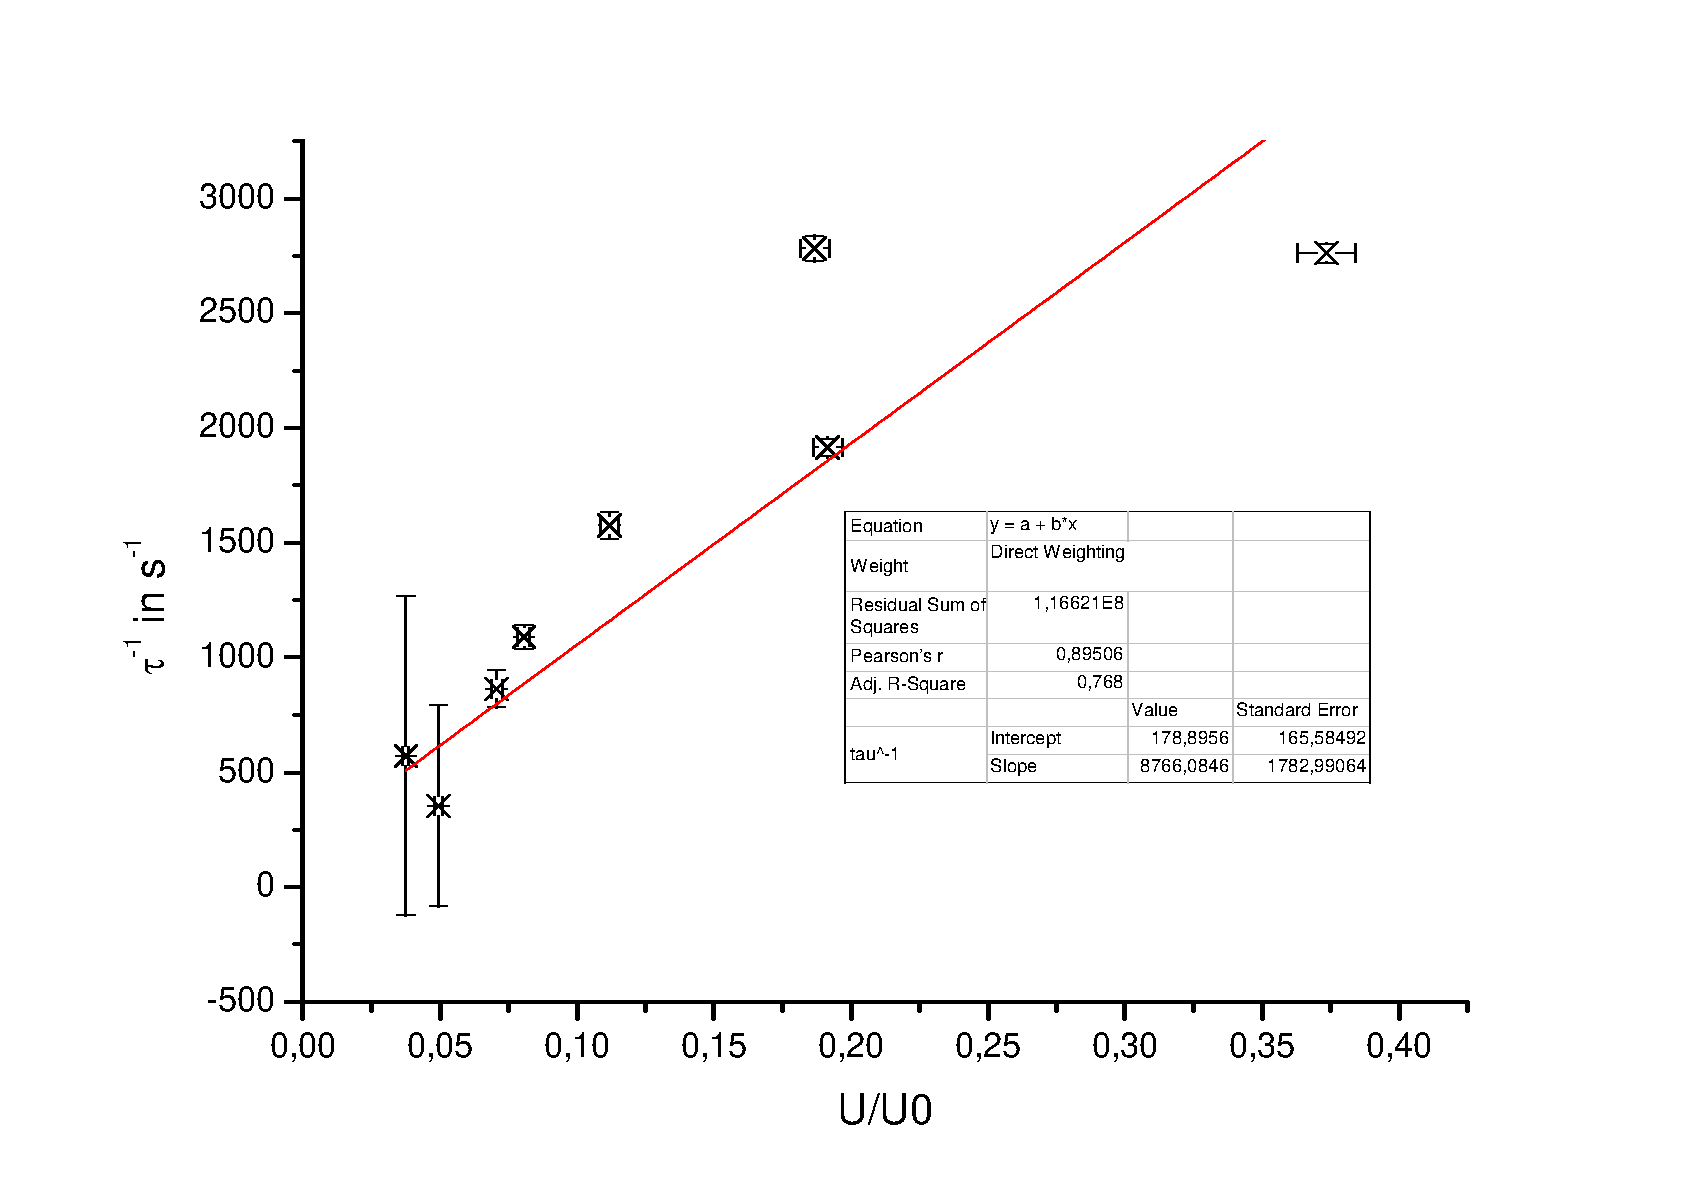
\includegraphics[width=\textwidth]{BilderAusw/Dehmelt.pdf}
\caption{Determination of the Relaxation time}
\end{figure}

From the fit, we can read, that the intercept with the y-axis is at $\tau^{-1} = (178.90 \pm 165.58)\ s^{-1}$. So we find the relaxation time:

$$\boxed{T_R = (5.590 \pm 5.174)\ ms}$$ \\

This value lies in the correct range which should be about in between 1 and 6 ms. Our value is so high because in our case the cell was very hot, since we constantly blow-dryed it. This is also the cause for the big value of the standard deviation, which is almost as large as the value itself. One can see in the plot, that most of the points don't really lie on the linear fit, too. We guess, that the plot and the values would have been much clearer without the constant blow-drying, however without it, the absorption was much less pronounced and harder to evaluate (\emph{see image \ref{dehmeltbsp} for reference}).

\subsection{Relaxation Time (Franzen)}

We tried a different method to determine the relaxation time of the Rubidium atoms, namely the method of Franzen. For this method, we also compensated the earth's vertical magnetic field using the induction coil 4. We set the laser to resonance ($I=64.4 mA$) and turned on the induction coil 1 in order to be able to fine-tune it. The temperature was set to $T=34.4^\circ C$.\\

\begin{figure}[H]
\begin{minipage}{0.5\textwidth}
\centering 
\includegraphics[width=0.5\textwidth]{BilderAusw/chopper.png}
\caption{A chopper disc [scitec.uk.com]}
\end{minipage}
\begin{minipage}{0.5\textwidth}
We inserted a rotating chopper disc into the optical path, which cut off the laser beam periodically. The laser pumped the Rubidium into the maximal polarization state. When the laser was blocked by the chopper disc, the Rubidium atoms had time to relax. By letting the laser pass through the disc again, one was able to see absorption lines.\\

\end{minipage}
\end{figure}

An absorption line looks like this:

\begin{figure}[H]
\centering 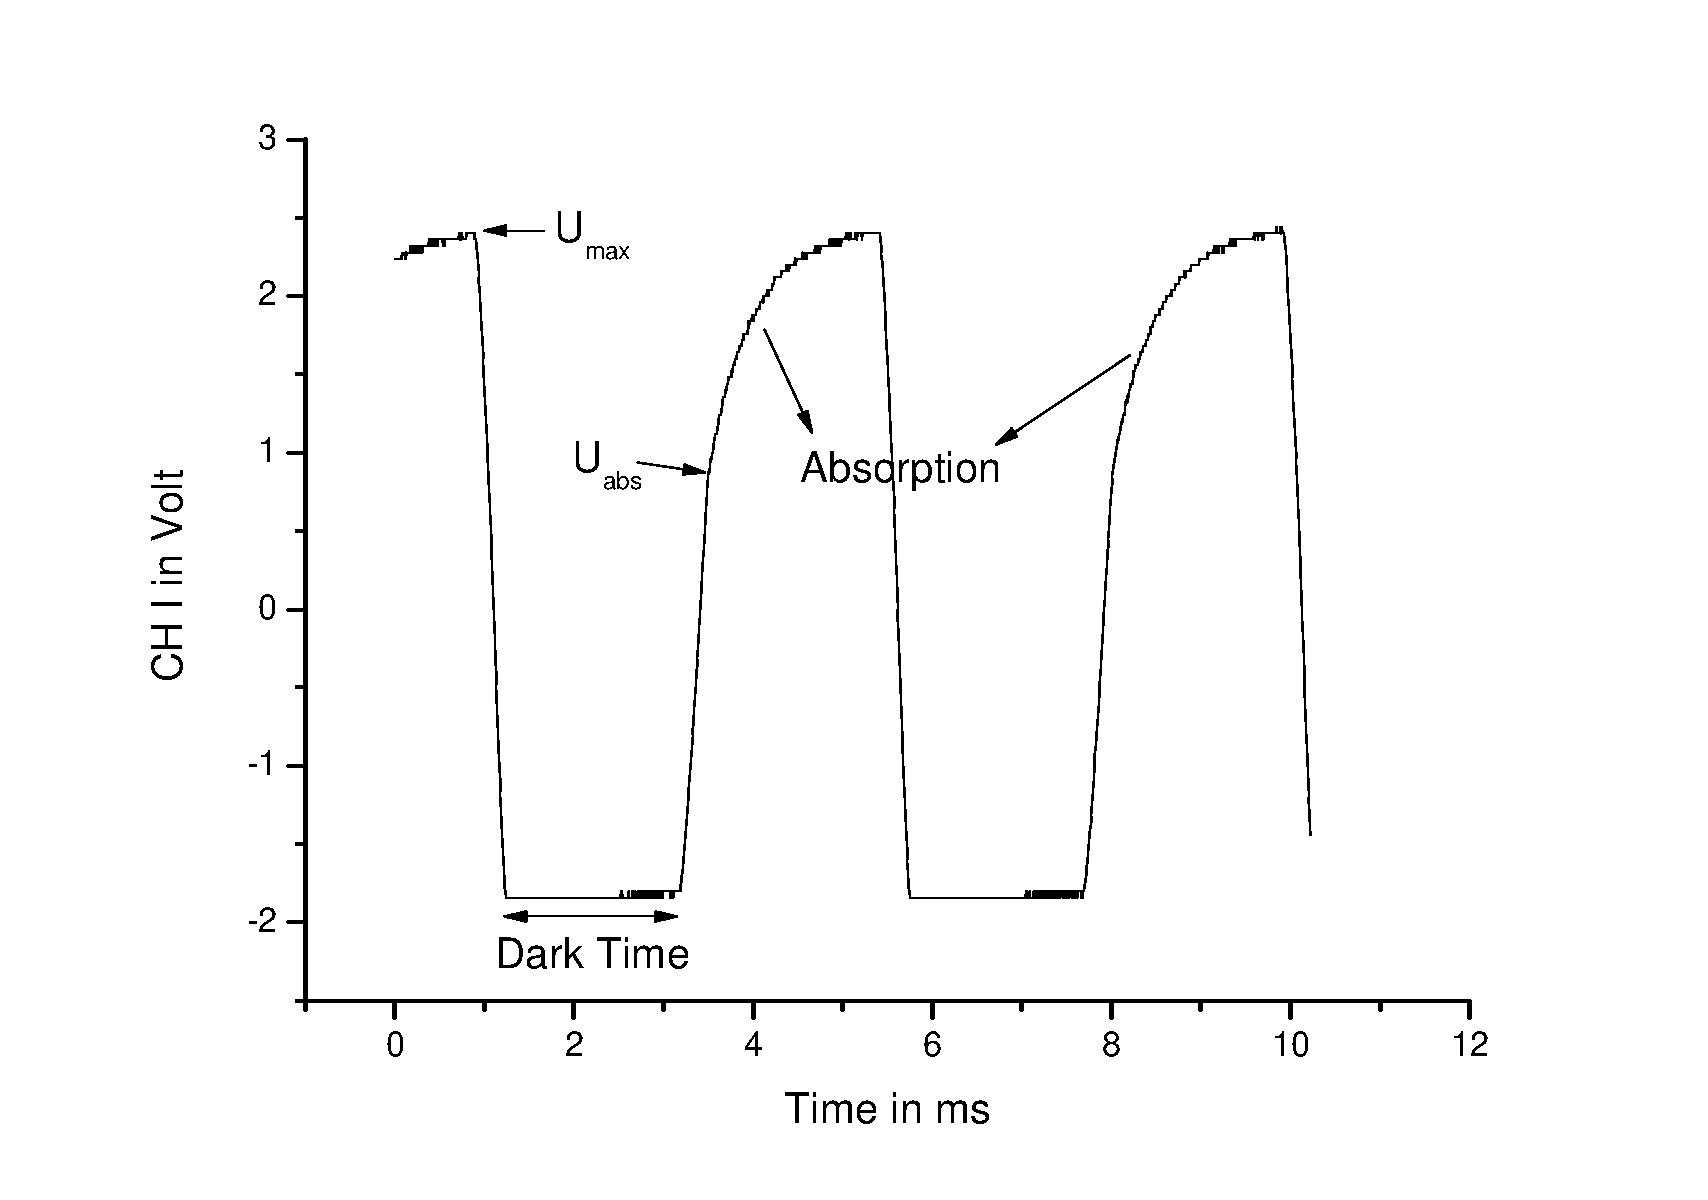
\includegraphics[width=\textwidth]{BilderAusw/FranzenBsp.pdf}
\caption{Absorption line with Franzen's method}
\end{figure}





















